\documentclass[aspectratio=169,10pt]{beamer}
\usetheme[progressbar=frametitle,numbering=fraction,block=fill]{metropolis}
\usepackage[sfdefault,lining]{FiraSans}
\usepackage[T1]{fontenc}
\usepackage{amsmath,amssymb}
\usepackage{booktabs}
\usepackage{tikz}
\usetikzlibrary{arrows.meta,positioning}
\definecolor{gaC}{HTML}{2A78D6}
\definecolor{tsC}{HTML}{EB6834}
\definecolor{maC}{HTML}{1BAF7A}
\definecolor{vio}{HTML}{6250D6}
\definecolor{ink}{HTML}{0B0B0B}
\definecolor{ink2}{HTML}{52514E}
\definecolor{soft}{HTML}{F4F8FD}
\setbeamercolor{frametitle}{bg=ink,fg=white}
\setbeamercolor{progress bar}{fg=tsC,bg=ink2!30}
\setbeamercolor{normal text}{fg=ink}
\setbeamercolor{alerted text}{fg=tsC}
\setbeamercolor{block title}{bg=soft,fg=ink}
\setbeamercolor{block body}{bg=soft}
\setbeamerfont{frametitle}{size=\large}
\setlength{\leftmargini}{1.2em}
\newcommand{\fig}[2][\textwidth]{\begin{center}\includegraphics[width=#1,height=0.80\textheight,keepaspectratio]{../figures/slides/#2.pdf}\end{center}}
\newcommand{\bignum}[1]{{\Large\bfseries #1}}
\newcommand{\soft}[1]{{\small\color{ink2}#1}}

\title{Drones, Deadlines and NP-Hardness}
\subtitle{Crossing-aware metaheuristics for a capacitated medical delivery network over the Bosphorus}
\author{Faruk Alpay \quad {\small 2267273}}
\institute{CMP3005 Analysis of Algorithms \textperiodcentered{} Bah\c{c}e\c{s}ehir University \textperiodcentered{} Dr.\ G\"unet Ero\u{g}lu}
\date{Term project \textperiodcentered{} December 2026}

\begin{document}
\maketitle

% ------------------------------------------------------------------
\begin{frame}{MediDrone Istanbul: the morning question}
\fig{instances}
\vspace{-2mm}
\begin{center}
\soft{Every clinic exactly once \textperiodcentered{} payload $\le Q$ \textperiodcentered{} at most $K$ drones \textperiodcentered{}
every crossing of the strait costs $+P$}
\end{center}
\end{frame}

% ------------------------------------------------------------------
\begin{frame}{Why we will not solve it exactly every morning}
\vspace{4mm}
\begin{center}
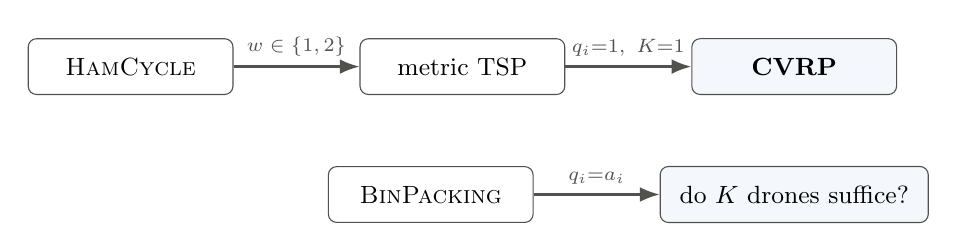
\begin{tikzpicture}[font=\small, box/.style={draw=ink2,rounded corners=3pt,inner sep=7pt,fill=white,minimum width=2.6cm},
  ar/.style={-{Latex[length=2.5mm]},thick,ink2}]
\node[box] (h) {\textsc{HamCycle}};
\node[box,right=1.6cm of h] (t) {metric TSP};
\node[box,right=1.6cm of t,fill=soft] (c) {\textbf{CVRP}};
\draw[ar] (h) -- node[above,font=\scriptsize]{$w\in\{1,2\}$} (t);
\draw[ar] (t) -- node[above,font=\scriptsize]{$q_i{=}1,\ K{=}1$} (c);
\node[box,below=0.9cm of c,fill=soft] (f) {do $K$ drones suffice?};
\node[box,left=1.6cm of f] (b) {\textsc{BinPacking}};
\draw[ar] (b) -- node[above,font=\scriptsize]{$q_i{=}a_i$} (f);
\end{tikzpicture}
\end{center}
\vspace{6mm}
\begin{columns}[T,onlytextwidth]
\column{0.32\textwidth}\centering\textbf{in NP}\\\soft{a plan is checked in $O(n)$}
\column{0.32\textwidth}\centering\textbf{strongly NP-complete}\\\soft{already for metric distances in $\{1,2\}$}
\column{0.32\textwidth}\centering\textbf{\alert{feasibility is hard too}}\\\soft{so the search may visit infeasible plans}
\end{columns}
\end{frame}

% ------------------------------------------------------------------
\begin{frame}{The Bosphorus is a cut metric}
\begin{columns}[c,onlytextwidth]
\column{0.5\textwidth}
\[
d(i,j)=e(i,j)+P\cdot\underbrace{[\,i,j\text{ on different sides}\,]}_{\text{cut semimetric }\delta_S}
\]
\vspace{2mm}
\begin{itemize}
\item metric for \alert{any} shoreline (real coastline too)
\item a closed route crosses an \alert{even} number of times
\item crossing routes $\ge$ Bin-Packing bound $\lceil q(\text{far})/Q\rceil$
\end{itemize}
\column{0.45\textwidth}
\begin{block}{Counter-examples}
\small
$\times$ multiplicative surcharge $e\,(1+\alpha\delta_S)$ breaks the triangle inequality\\[2pt]
$\times$ CVRPLIB rounding: 0.21\,\% of triples violate it
\end{block}
\end{columns}
\end{frame}

% ------------------------------------------------------------------
\begin{frame}{Data: benchmark, synthetic and real}
\begin{columns}[T,onlytextwidth]
\column{0.24\textwidth}\centering \bignum{74+11}\\ \soft{CVRPLIB A/B/P/X\\ via Hugging Face}
\column{0.24\textwidth}\centering \bignum{seed 7273}\\ \soft{team instance\\ $n=100$, $K=18$}
\column{0.24\textwidth}\centering \bignum{905}\\ \soft{real OSM facilities\\ in Istanbul}
\column{0.24\textwidth}\centering \bignum{9}\\ \soft{tiny instances, exact\\ by DP $=$ MILP}
\end{columns}
\vspace{8mm}
\begin{center}
\soft{Independent Python checker re-validates every reported solution (capacity, each clinic once, $\le K$, cost).}
\end{center}
\end{frame}

% ------------------------------------------------------------------
\begin{frame}{Three algorithms}
\begin{columns}[T,onlytextwidth]
\column{0.32\textwidth}
\textbf{Clarke--Wright}\\[2pt]
\soft{savings, $\Theta(n^2\log n)$\\ baseline \& TS start}
\column{0.32\textwidth}
\textbf{\color{gaC}GA} / \textbf{\color{maC}MA}\\[2pt]
\soft{giant tour + optimal Split\\ OX, mutation, clone rejection\\ MA: + local search}
\column{0.32\textwidth}
\textbf{\color{tsC}Tabu Search}\\[2pt]
\soft{4 neighbourhoods, $O(1)$ deltas\\ tabu edges, aspiration\\ adaptive overload penalty}
\end{columns}
\vspace{5mm}
\begin{center}\includegraphics[width=\textwidth]{tikz/split.pdf}\end{center}
\begin{center}\soft{Split $=$ shortest path in a DAG: $\Theta(nL)$ Bellman, or $\Theta(n)$ with a monotone deque}\end{center}
\end{frame}

% ------------------------------------------------------------------
\begin{frame}{Tabu search: four neighbourhoods, $O(1)$ each}
\vspace{3mm}
\begin{center}\includegraphics[width=0.92\textwidth]{tikz/moves.pdf}\end{center}
\vspace{4mm}
\begin{columns}[T,onlytextwidth]
\column{0.32\textwidth}\centering\textbf{granular}\\\soft{$v\in N_{20}(u)$: $\le 7nk+n$ moves}
\column{0.32\textwidth}\centering\textbf{tabu edges}\\\soft{random tenure $[10,25]$, aspiration}
\column{0.32\textwidth}\centering\textbf{strategic oscillation}\\\soft{$\lambda\cdot$overload, $\lambda(1\pm0.3)$}
\end{columns}
\end{frame}

% ------------------------------------------------------------------
\begin{frame}{Complexity: theory meets the stopwatch}
\fig{complexity}
\begin{center}\soft{TS iteration $\Theta(nk)$: slope 1.08 \textperiodcentered{} full neighbourhood $\Theta(n^2)$: 2.12 \textperiodcentered{}
$O(n)$ Split is $37\times$ faster than Bellman at $L=500$}\end{center}
\end{frame}

% ------------------------------------------------------------------
\begin{frame}{Results on the required instances}
\begin{center}
\begin{tabular}{@{}l r r r r@{}}
\toprule
mean gap (\%) \quad [runs at best] & CW & \textcolor{gaC}{GA} & \textcolor{maC}{MA} & \textcolor{tsC}{TS} \\
\midrule
A-n32-k5 & 7.40 & 5.48 [0] & \textbf{0.00 [10]} & \textbf{0.00 [10]} \\
A-n45-k6 & 5.61 & 1.15 [3] & \textbf{0.00 [10]} & \textbf{0.00 [10]} \\
A-n60-k9 & 3.99 & 3.12 [0] & \textbf{0.00 [10]} & \textbf{0.00 [10]} \\
A-n80-k10 & 4.37 & 3.12 [0] & \textbf{0.00 [10]} & 0.03 [6] \\
MediDrone-7273 & 8.92 & 3.03 [0] & 0.05 [7] & \textbf{0.01 [9]} \\
MediDrone-IST-7273 & 2.74 & 1.59 [0] & \textbf{0.04 [7]} & 0.07 [2] \\
\bottomrule
\end{tabular}

\end{center}
\vspace{2mm}
\begin{center}\soft{10 seeds, equal wall-clock budgets (30/60\,s) \textperiodcentered{} TS $\succ$ GA on every instance ($p\le0.002$)}\end{center}
\end{frame}

% ------------------------------------------------------------------
\begin{frame}{Anytime behaviour}
\vspace{2mm}
\fig{convergence_top}
\begin{center}\soft{TS starts from the repaired CW plan and is at the optimum within 1\,ms on A-n45-k6 \textperiodcentered{} MA overtakes on A-n80-k10 \textperiodcentered{} GA improves slowly}\end{center}
\end{frame}

% ------------------------------------------------------------------
\begin{frame}{When is a plan good enough? Attainment functions}
\vspace{2mm}
\fig{convergence_eaf}
\begin{center}\soft{``within 1\,\% after 1\,s'': every TS and MA run, no GA run \textperiodcentered{} median TS run within 0.1\,\% after 4.1\,s}\end{center}
\end{frame}

% ------------------------------------------------------------------
\begin{frame}{The plans}
\fig{routes}
\begin{center}\soft{crossing routes $=$ Bin-Packing bound on both instances \textperiodcentered{} no route ever zig-zags}\end{center}
\end{frame}

% ------------------------------------------------------------------
\begin{frame}{What the strait does}
\vspace{1mm}
\fig[0.95\textwidth]{psweep_maps}
\vspace{2mm}
\begin{columns}[T,onlytextwidth]
\column{0.48\textwidth}
\textbf{Team instance: same plan for every $P$}\\[2pt]
\soft{The $P=0$ optimum already uses the minimum 10 crossings, so it stays optimal (corollary); cost $=17\,724+20P$.}
\column{0.48\textwidth}
\textbf{Istanbul: $7\to6$ crossings at $P^\ast=1.12$\,km}\\[2pt]
\soft{Predicted from the two competing plans (566.97 vs 569.21\,km, 14 vs 12 crossings); measured switch between 1 and 2\,km.}
\end{columns}
\end{frame}

% ------------------------------------------------------------------
\begin{frame}{Why TS and MA beat GA}
\fig{stn}
\begin{center}\soft{Only methods that \alert{relocate clinics between routes} funnel into the optimal partition.}\end{center}
\end{frame}

% ------------------------------------------------------------------
\begin{frame}{Beyond four instances}
\vspace{1mm}
\fig{extended}
\begin{center}\soft{Wilcoxon signed-rank over 74 instances: TS vs GA $p=1.6\cdot10^{-11}$ \textperiodcentered{} TS vs MA $p=0.218$
}\end{center}
\end{frame}

% ------------------------------------------------------------------
\begin{frame}{When feasibility itself is hard}
\vspace{6mm}
\begin{columns}[c,onlytextwidth]
\column{0.42\textwidth}\centering
{\Huge\bfseries 0.992}\\[2pt]\soft{load factor of P-n55-k15\\($\sum q = 1042$ for $K\cdot Q = 1050$)}
\column{0.55\textwidth}
\begin{itemize}
\item \textbf{\color{gaC}GA}, \textbf{\color{maC}MA}: no plan with $\le K$ drones in \alert{any} run
\item \textbf{\color{tsC}TS}: optimum 989 in \alert{every} run
\item Clarke--Wright exceeds the fleet on 25 of 74 instances
\end{itemize}
\end{columns}
\vspace{8mm}
\begin{center}\soft{Theorem: deciding whether $K$ drones suffice is Bin Packing --- walking through infeasible space pays off.}\end{center}
\end{frame}

% ------------------------------------------------------------------
\begin{frame}{Three lessons}
\vspace{4mm}
\begin{enumerate}\setlength{\itemsep}{10pt}
\item \textbf{Hardness hides in feasibility.} Even ``do $K$ drones suffice?'' is Bin Packing --- and it bites on real benchmarks.
\item \textbf{Moves matter more than populations.} Relocating clinics between routes is what finds the optimal partition.
\item \textbf{Theory predicts the data.} The crossing bound is attained; the Istanbul switch at $P^\ast=1.12$\,km was predicted.
\end{enumerate}
\vspace{6mm}
\soft{Surprise: the Clarke--Wright seed can trap the GA --- on A-n32-k5 all 10 seeded runs end at 827, unseeded runs reach 784 in 8 of 10.}
\end{frame}

% ------------------------------------------------------------------
\begin{frame}[standout]
Thank you\\[6pt]
{\normalsize everything reproducible with one command}
\end{frame}
\end{document}
